% used inside TikZ, thus must be accessible to PlasTeX as well
\usepackage[dvipsnames]{xcolor}

% HTML from website SASS
\definecolor{mbrpBlue}{HTML}{336699}
\definecolor{mbrpOrange}{HTML}{ff9300}
\colorlet{mbrpBlueBg}{mbrpBlue!20}
\colorlet{mbrpOrangeBg}{mbrpOrange!20}
% semantic foreground
\colorlet{mbrpAuto}{mbrpBlue}
\colorlet{mbrpSober}{mbrpOrange}
% semantic background
\colorlet{mbrpAutoBg}{mbrpAuto!20}
\colorlet{mbrpSoberBg}{mbrpSober!20}


\newcommand*\cleartoleftpage{%
  \clearpage
  \ifodd\value{page}\thispagestyle{empty}\hbox{}\newpage\fi
}


\usepackage{tikz}
\usetikzlibrary{
	matrix,fit,shapes.callouts,shapes.arrows,shapes.misc,positioning,decorations.pathmorphing,arrows.meta,fpu,shapes.multipart,mindmap,arrows
}


% https://tex.stackexchange.com/a/72793
\tikzset{
	outlined arrow/.style args={#1 colored by #2 and #3}{
		-latex,
		line width=#1,color=#2,
		postaction={draw,-latex,color=#3,line width=(#1)/3,shorten <=(#1)/4,shorten >=4.5*(#1)/3}
	}
}

% https://tex.stackexchange.com/a/61362/6758
\tikzset{
	every fit/.append style=text badly centered,
}

% https://tex.stackexchange.com/a/8473/6758
\newcommand*\circled[1]{\tikz[baseline=(char.base)]{
    \node[shape=circle,draw,inner sep=2pt] (char) {#1};
}}

%\tikzset{
%  disable rounded corners for decorations/.style={
%    /pgf/every decoration/.style={
%      /tikz/sharp corners
%    },
%  }
%}

\tikzset{>=latex}

\tikzset{
	% custom asymetric columnns
	left column/.style args={below #1}{at=(#1.south),anchor=north east,shift=({-.5em,-1em})},
	right column/.style args={below #1}{at=(#1.south),anchor=north west,shift=({.5em,-1em})},
	narrower left column/.style args={below #1}{at=(#1.south),anchor=north east,shift=({-.5em-.15\linewidth,-1em})},
	wider right column/.style args={below #1}{at=(#1.south),anchor=north west,shift=({.5em-.15\linewidth,-1em})},
	% custom styles
	thought/.style={dashed,rounded corners,font=\itshape},
	action/.style={solid,sharp corners},
	% FIXME: why not 2\pgfkeysvalueof{/pgf/inner xsep} ??
	wider sober/.style={
		fill=mbrpSoberBg,align=justify,dotted,rectangle split,rectangle split parts=2,sharp corners,
		text width=.65*(\linewidth-1em)-1*\pgfkeysvalueof{/pgf/inner xsep}-2*\pgflinewidth
	},
	sober/.style={fill=mbrpSoberBg,align=justify,dotted,rectangle split,rectangle split parts=2,sharp corners},
	mindful/.style={fill=mbrpSoberBg,align=center,dotted},
	narrower autopilot/.style={
		fill=mbrpAutoBg,
		text width=.35*(\linewidth-1em)-1*\pgfkeysvalueof{/pgf/inner xsep}-2*\pgflinewidth
	},
	autopilot/.style={fill=mbrpAutoBg,dashed},
	sober arrow/.style={outlined arrow={.5mm colored by black and mbrpSoberBg}},
	wide sober arrow/.style={outlined arrow={1mm colored by black and mbrpSoberBg}},
	autopilot arrow/.style={outlined arrow={.5mm colored by black and mbrpAutoBg}},
	wide autopilot arrow/.style={outlined arrow={1mm colored by black and mbrpAutoBg}},
}

\def\soberName#1{\textbf{#1} \nodepart{two} }

\def\mbrpset#1{\pgfkeys{/mbrp/.cd,#1}}
\pgfkeys{/mbrp/.is family,/mbrp,
	title1/.initial=\undefined,
	title2/.initial=\undefined,
	autopilot/.store in=\mbrpAutopilot,
	sober S/.initial={Zastavte se a vyskočte z autopilota.},
	sober O/.store in=\mbrpBrzdaR,
	sober O/.initial=\undefined,
	sober B/.initial={Několikrát se pomalu a pozorně nadýchěte a vydýchněte. Pozornost zaměřte na dech.},
	sober E/.initial={Rozšiřte znovu svou pozornost na to, jak se cítíte. Nakolik to jde, zkuste to udělat s postojem otevřenosti a přijetí.},
	sober R/.store in=\mbrpBrzdaA,
	sober R/.initial=\undefined,
	%
	title/.initial=\undefined,
	title/.store in=\mbrpTitle,
	toc title/.initial=\relax,
	toc title/.store in=\mbrpTocTitle,
	summary/.initial=\undefined,
	informal moments/.initial=\undefined,
	informal challenges/.initial=\undefined,
	informal activities/.initial=\undefined,
	formal/.initial=\undefined,
	practice sheets/.initial=\undefined
}

\newcommand{\mbrpSession}[1]{
	\bgroup
	\let\mbrpTocTitle\relax
	\mbrpset{#1}
	\cleardoublepage
	\addtocounter{section}{1}
	\setcounter{subsection}{0}
	\ifx\mbrpTocTitle\relax\let\mbrpTocTitle\mbrpTitle\fi
	\xdef\toct{\arabic{section}. \mbrpTocTitle}
	\sectionmark{\mbrpTocTitle}
	\addcontentsline{toc}{section}{\toct}
	\thispagestyle{start-session}
	\bgroup
		\null\vskip1cm minus 1cm
		\begin{tcolorbox}[
			skin=bicolor,
			boxrule=.4pt,
			coltitle=black,
			colbacktitle=mbrpBlueBg,
			colback=white,
			parbox=false,
			adjusted title={\textbf{\Large\strut \arabic{section}. setkání}},
			% subtitle style={before={\vspace*{-1ex}}}
			%frame hidden,
		]
			\vskip1em
			{ \scshape\bfseries\Large\strut \mbrpTitle }
			\vskip1.5em
			\tcbsubtitle{{\large\strut \textbf{Shrnutí}}}
			\vskip.5em
			{\let\item\par \par\pgfkeysvalueof{/mbrp/summary}\par}
			\vskip.5em
		\end{tcolorbox}

		\clearpage

		\begin{tcolorbox}[
			skin=bicolor,
			boxrule=.4pt,
			%frame hidden,
			title={\strut Formální cvičení},
			parbox=false,
			coltitle=black,
			colbacktitle=mbrpOrangeBg,
			colback=white,
			fonttitle=\bfseries\large,
			% subtitle style={before={\vspace*{-1ex}}}
		]
			Snažte se poslouchat nahrávky vedených cvičení všímavosti každý den či obden (4× až 6× za týden). Vyzkoušejte cvičit pokaždé ve stejnou dobu (např. před snídaní).

			Do dalšího sezení doporučujeme se zaměřit na cvičení:
				\begin{itemize*}
					\pgfkeysvalueof{/mbrp/formal}
				\end{itemize*}
			\medskip
			\tcbsubtitle{\strut Neformální cvičení} % , za pochodu}
				\begin{description}
					\item[Okamžiky:] \pgfkeysvalueof{/mbrp/informal moments}
					\item[Obtíže:]   \pgfkeysvalueof{/mbrp/informal challenges}
					\item[Činnosti:] \pgfkeysvalueof{/mbrp/informal activities}
				\end{description}
			\tcbsubtitle{\strut Pracovní listy \normalPencilLeftDown}
				\begin{itemize*}
					\pgfkeysvalueof{/mbrp/practice sheets}
					\item záznam denního cvičení.
				\end{itemize*}
				\medskip
		\end{tcolorbox}
	\egroup
	\clearpage
	\egroup
}


\newcommand{\soberSpace}[1]{
	\begin{adjustbox}{width=\linewidth,height=.9\textheight,keepaspectratio}
	\begin{tikzpicture}[
		every node/.style={
			align=center,
			text width=(\linewidth-1em)/2-2*\pgfkeysvalueof{/pgf/inner xsep}-2*\pgflinewidth,
			draw,
			rounded corners,
		},
		node distance=1em,
	]
	\mbrpset{#1}

	\node(top)[text width=.9\linewidth,text badly centered]{ \textsc{\pgfkeysvalueof{/mbrp/title1}} \\ \pgfkeysvalueof{/mbrp/title2} };
	\node(a0)[narrower autopilot, narrower left column=below top]{a0};
	\node(a0)[narrower autopilot,draw=none,narrower left column=below top]{$\downarrow${} \textsc{Autopilot} $\downarrow$};
	\draw[autopilot arrow] (top)--(a0);
	\foreach [var=\type,var=\content,count=\curr,remember=\curr as \prev (initially 0)] in \mbrpAutopilot {
		\node(a\curr) [narrower autopilot,\type,below=of a\prev]{\content};
		\draw[autopilot arrow] (a\prev.south)--(a\curr.north);
	}


	\node(b1)[wider sober,wider right column=below top]{\soberName{Brzdi!} \pgfkeysvalueof{/mbrp/sober S}};
	\node(b2)[wider sober,below=of b1]{\soberName{Roz-vhled!} Podívejte se bez posuzování na probíhající zkušenost: \begin{iitemize}\foreach\content in\mbrpBrzdaR{\item\content}\end{iitemize}};
	\node(b3)[wider sober,below=of b2]{\soberName{Zakotvi se!} \pgfkeysvalueof{/mbrp/sober B}};
	\node(b4)[wider sober,below=of b3]{\soberName{Doširoka se otevři!} \pgfkeysvalueof{/mbrp/sober E}};
	\node(b5)[wider sober,below=of b4]{\soberName{Akce!} Jednejte z porozumění situaci, které máte. \begin{iitemize}\foreach\content in\mbrpBrzdaA{\item\content}\end{iitemize}};
	\begin{scope}
		\draw[sober arrow] (top) -- (b1);
		\draw[sober arrow] (b1) -- (b2);
		\draw[sober arrow] (b2) -- (b3);
		\draw[sober arrow] (b3) -- (b4);
		\draw[sober arrow] (b4) -- (b5);
	\end{scope}
	\end{tikzpicture}
	\end{adjustbox}
}

\newcommand{\soberSpaceEmpty}[1]{
	%\begin{adjustbox}{width=\linewidth,height=.85\textheight,keepaspectratio}
	\mbrpset{#1}
	\def\miniStrut{\rule[-.4ex]{0pt}{0pt}}
	\def\thoughtsFeelingsActions{\leavevmode\lower.3ex\hbox{\vbox{\tiny\baselineskip=0pt\lineskip=-.3ex\hbox{myšlenky}\hbox{pocity}\hbox{jednání}}}}
	\def\bodyFeelingsMind{\leavevmode\lower.3ex\hbox{\vbox{\tiny\baselineskip=0pt\lineskip=-.3ex\hbox{tělo\miniStrut}\hbox{pocity\miniStrut}\hbox{mysl\miniStrut}}}}
	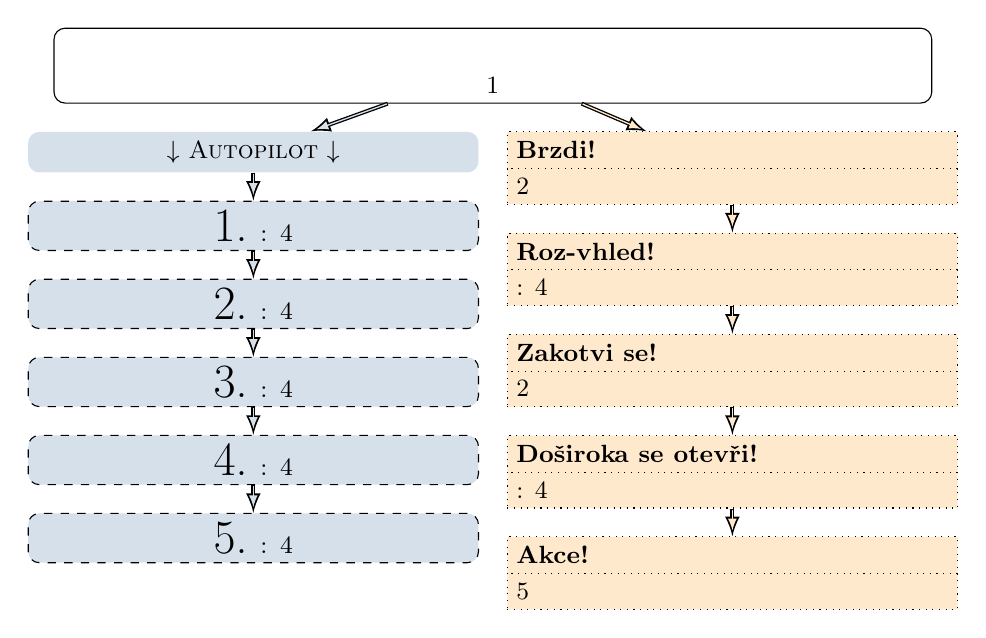
\begin{tikzpicture}[
		every node/.style={
			align=center,
			text width=(\linewidth-1em)/2-2*\pgfkeysvalueof{/pgf/inner xsep}-2*\pgflinewidth-4pt,
			% minimum width=(\linewidth-1em)/2, %-2*\pgfkeysvalueof{/pgf/inner xsep}-2*\pgflinewidth,
			draw,
			rounded corners,
			font=\small
		},
		node distance=1em,
	]
	\node(top)[text width=.9\linewidth]{\textsc{\pgfkeysvalueof{/mbrp/title1}} \\ \rule{0em}{5ex}\Blank{1}};
	\node(a0)[autopilot,draw=none,left column=below top]{$\downarrow${} \textsc{Autopilot} $\downarrow$};
	\draw[autopilot arrow] (top)--(a0);
	\foreach [var=\curr,remember=\curr as \prev (initially 0)] in {1,2,3,4,5} {
		\node(a\curr) [autopilot,below=of a\prev]{{\LARGE \curr.} \thoughtsFeelingsActions: \Blank{4}};
		\draw[autopilot arrow] (a\prev.south)--(a\curr.north);
	}


	\node(b1)[sober,right column=below top]{\soberName{Brzdi!} \Blank{2}};
	\node(b2)[sober,below=of b1]{\soberName{Roz-vhled!} \bodyFeelingsMind: \Blank{4}};
	\node(b3)[sober,below=of b2]{\soberName{Zakotvi se!} \Blank{2}};
	\node(b4)[sober,below=of b3]{\soberName{Doširoka se otevři!} \bodyFeelingsMind: \Blank{4}};
	\node(b5)[sober,below=of b4]{\soberName{Akce!} \Blank{5}};

	\begin{scope}
		\draw[sober arrow] (top) -- (b1);
		\draw[sober arrow] (b1) -- (b2);
		\draw[sober arrow] (b2) -- (b3);
		\draw[sober arrow] (b3) -- (b4);
		\draw[sober arrow] (b4) -- (b5);
	\end{scope}
	\end{tikzpicture}
	%\end{adjustbox}
}

\def\pageSOBERown#1#2{
	% \clearpage\subsection*{#1 \normalPencilLeftDown}
	\vskip-1em #1{} Co se pak stane, když fungujete na autopilota? Jak byste v takové situaci mohli použít \textsc{Brzd}u? Do každého kroku \textsc{Brzd}y vlastními slovy vepište, co byste udělali či vnímali.\par
	\vskip0pt minus1cm
	\soberSpaceEmpty{title1={#2}}
}



\def\pageGuesthouse{
	\clearpage
\subsection{Dům pro hosty\footnote{Autor překladu neznámý.}}
	%[\emph{Rúmí}; autor překladu neznámý]
	% FROM https://tex.stackexchange.com/a/196934/6758
	\newlength{\saveleftmargini}
	\setlength{\saveleftmargini}{\leftmargini}
	\setlength{\leftmargini}{0em}
	\begin{verse}
	Lidská bytost je jako dům pro hosty.\\
	Každé ráno přicházejí noví hosté.

	Radost, zármutek, podlost, \\
	okamžitý stav mysli přichází \\
	jako nečekaný host.

	Všechny přivítej a bav se s nimi! \\
	I když je to je houf starostí, \\
	které vtrhnou dovnitř a násilím rabují.

	I přesto přivítej každého hosta s úctou. \\
	Možná tě zbaví něčeho, \\
	co ti bránilo prožít nové radosti.

	Temné myšlenky, stud a zlobu \\
	přivítej s úsměvem u dveří \\
	a pozvi je dál.

	Za každého, kdo přijde, buď vděčný, \\
	protože ti jej osud posílá \\
	jako učitele.
	\end{verse}
	\setlength{\leftmargini}{\saveleftmargini}
	\hskip.5\linewidth\emph{Rúmí}
	% \vfill
}


\def\pageSOBER{
	\subsection{\textsc{Brzda}}
		\textsc{Brzda} \emph{je cvičení všímavosti „za pochodu“, které můžete použít kdekoliv a kdykoliv, protože je krátké, jednoduché a přizpůsobivé.} Můžete ho udělat za pár sekund i mu dát několik minut. Lze ho použít ve stresující situaci, když jste rozčilení či zakoušíte nutkání či vnitřní impulsy k jednání, kterému se chcete vyhnout. Je užitečné, i když jde všechno hladce, cítíte se dobře, či kdykoliv chcete být duchem „více tady“ k ocenění odehrávající se přítomnosti. Může vám pomoci k vyskočení z reaktivního autopilota a být si víc vědomý v tom, jak v nastalé situaci budete jednat.

		\begin{itemize}
		\itemStop{B}{Brzdi.} Šlápněte na brzdu a zastavte se, abyste toto cvičení mohli udělat. Je to první krok, kterým vystoupíte z autopilota.
		\itemStop{R}{Roz-vhled.} Rozhlédněte se uvnitř sebe, ve své svou momentální zkušenosti, a rozeberte ji na části: tělesné počitky, pocity, myšlenky. Zkuste se na ně podívat s určitou zvědavostí a bez odsuzování.
		\itemStop{Z}{Zakotvi se.} Udělejte několik pomalých nádechů a výdechů a zakotvěte přitom svou pozornost v tělesných počitcích, které dýchání doprovázejí.
		\itemStop{D\kern-.1em}{Doširoka se otevři.} Rozšiřte pozornost od dechu na celé tělo a pak i na celou situaci, ve které se nacházíte.
		\itemStop{A}{Akce.} Jednete v nastalé situaci s vnitřní orientací, nenechte jen proběhnout automatickou reakci. Buďte aktivní, ne reaktivní. Uvědomte si, že ve svém jednání máte na výběr. Zamyslete se nad tím, co v tuto chvíli potřebujete a jak byste se o sebe nejlépe postarali.
		\end{itemize}
	}

	\def\pagePracticeLog{
		%\par\vfill\pagebreak % this will acutally flush the previous page (unlike clearpage) and \newgeometry won't affect the previous page
		%\newgeometry{right=1cm,bottom=1cm} % top=1cm,left=1cm
		\practiceSheetTitle{Záznam cvičení}
		%\enlargethispage{5cm}
		\bgroup
			\def\myStrut{\rule{0pt}{\dimexpr(\pagewidth+5mm-8em-2cm-6em-3pt)/7}} % {.07\textheight}}
			\footnotesize
			%\noindent\kern-5mm
			\begin{adjustbox}{angle=90,Trim={10mm 50mm 0mm 5mm}}
			\begin{tblr}{
				width=\dimexpr\textheight+18mm\relax,
				colspec={X[l,1.3]|X[l,4]|X[l,4]|X[l,2]},
				%row{2}={font=\tiny}
			}
				{datum \\ den } & {
					\textbf{pravidelné cvičení} \\
					{\tiny čas vyhrazený na nahrávku} \\
					Co jsem cvičil? Jak dlouho?
				} & {
					\textbf{cvičení za pochodu}  \\
					\textbf{okamžiky}: náhodné napojení na sebe \\
					\textbf{obtíže}: \textsc{Brzda} v náročné situaci \\
					\textbf{činnosti}: jídlo, chůze, domácí práce, pohyb venku \\
					Co jsem dělal? Kolikrát?
				} & { poznámky \\ postřehy  } \\
				\hline \myStrut & \myStrut & \myStrut & \myStrut \\
				\hline \myStrut & \myStrut & \myStrut & \myStrut \\
				\hline \myStrut & \myStrut & \myStrut & \myStrut \\
				\hline \myStrut & \myStrut & \myStrut & \myStrut \\
				\hline \myStrut & \myStrut & \myStrut & \myStrut \\
				\hline \myStrut & \myStrut & \myStrut & \myStrut \\
				\hline \myStrut & \myStrut & \myStrut & \myStrut \\
			\end{tblr}
			\end{adjustbox}
		\egroup
		% \restoregeometry
	}



\def\pageBasicFeelings{
	\clearpage
	\subsection[Slovní zásoba pro pocity]{Slovní zásoba pro pocity\footnote{Podle \emph{Feelings and needs we all have} — \href{https://www.nonviolentcommunication.com/learn-nonviolent-communication/feelings/}{https://www.nonviolentcommunication.com/learn-nonviolent-communication/feelings/}.}}
		\label{slovni-zasoba-pocity}
		Můžete použít následující soupis jako inspiraci pro rozšíření palety pocitů, které v sobě dokážete rozpoznat a pojmenovat.

		\begin{multicols}{2}
		Při základní spokojenosti:
		\begin{itemize*}
			\item ohromení
			\item sebedůvěra
			\item energičnost
			\item potěšení
			\item inspirace
			\item radost
			\item optimistismus
			\item úleva
			\item překvapení
			\item dojetí
			\item pohodlí
			\item horlivost
			\item naplněnost
			\item být plný naděje
			\item být zaujatý
			\item pohnutí
			\item hrdost
			\item povzbuzení, stimulace
			\item vděčnost
			\item být plný důvěry
		\end{itemize*}
		\columnbreak
		Při základní nespokojenosti:
		\begin{itemize*}
			\item vztek
			\item zmatení
			\item zklamání
			\item zoufalství
			\item frustrace
			\item beznaděj
			\item podráždění
			\item nervozita
			\item zaseknutí
			\item smutek
			\item otrávenost
			\item znepokojení
			\item zhrzenost, odrazení
			\item zahanbenost
			\item bezmoc
			\item netrpělivost
			\item osamělost
			\item být přemožený děním
			\item neochota
			\item nepohoda
		\end{itemize*}
		\end{multicols}
}

\def\pageBasicNeeds{
	\subsection[Slovní zásoba pro potřeby]{Slovní zásoba pro potřeby\footnote{Podle \emph{Feelings and needs we all have} — \href{https://www.nonviolentcommunication.com/learn-nonviolent-communication/feelings/}{https://www.nonviolentcommunication.com/learn-nonviolent-communication/feelings/}.}}
		\label{slovni-zasoba-potreby}
		\setstretch{.95}
		Můžete použít následující soupis potřeb jako inspiraci pro rozšíření palety potřeb, které v sobě dokážete rozpoznat a pojmenovat.
		\begin{multicols}{2}
			\begin{itemize*}
				\item autonomie
					\begin{itemize*}
						\item vybírat si sny/cíle/hodnoty
						\item vybírat si plány pro naplnění svých snů, cílů, hodnot
					\end{itemize*}
				\item slavení
					\begin{itemize*}
						\item slavení výtvorů života a naplněných snů
						\item slavení ztrát: blízkých lidí, snů, … (truchlení)
					\end{itemize*}
				\item integrita
					\begin{itemize*}
						\item autenticita
						\item tvořivost, kreativita
						\item smysl
						\item sebehodnota
					\end{itemize*}
				\item propojenost
					\begin{itemize*}
						\item přijetí
						\item ocenění
						\item blízkost
						\item společenství
						\item ohleduplnost
						\item přispívat k obohacení života
						\item emoční bezpečí
						\item soucit, empatie
						\item upřímnost (posilující upřímnost, díky které se můžeme učit z vlastních omezení)
						\item láska
						\item ujištění
						\item respekt
						\item podpora
						\item důvěra
						\item porozumění
					\end{itemize*}
				\item péče o tělo
					\begin{itemize*}
						\item vzduch
						\item jídlo
						\item pohyb, cvičení
						\item ochrana před život ohrožujícími organismy: viry, bakteriemi, hmyzem, dravou zvěří
						\item odpočinek
						\item sexuální vyjádření
						\item přístřeší
						\item dotyk
						\item voda
					\end{itemize*}
				\item hra
					\begin{itemize*}
						\item zábava
						\item smích
					\end{itemize*}
				\item duchovní společenství
					\begin{itemize*}
						\item krása
						\item soulad, harmonie
						\item inspirace
						\item řád
						\item pokoj, mír
					\end{itemize*}
			\end{itemize*}
		\end{multicols}
}

